\chapter{A Simple Example: An Address Book}
\label{chap:simpleex}
% All figures in this chapter are available on the web in png format at:
%   http://www.usegantry.org/images/tenttut/{name}.png
% where {name} is the name of the eps file loaded here.

Most Gantry apps (and probably most web apps) are really database front ends.
This leads to a philosophy of web development: concentrate on the data model.
To have an example, consider my wife's address book.  Suppose I want to migrate
this to a web app, so she can more easily back it up and stop lugging it
around.  (I apologize to readers intimate with the project docs, for
whom this is all starting to sound strikingly familiar.  There are novel
examples in this book.  See the `Contact Us' and `Job Ads' case studies in
Part II.)

The initial data model for an address book is pretty simple, with just
one table having a row for each person or family.  We'll make it slightly
more interesting later, by allowing birthdays.

\section{Take One: Name and number please.}

There are many ways to build a one table web app.  Even if we limit ourselves
to Gantry, there are still several approaches.  I'm looking for the easiest
one here, never wanting my laziness to be doubted.  Therefore, I'll start with
bigtop generation:

\begin{verbatim}
bigtop --new AddressBook address
\end{verbatim}

(You may abbreviate all bigtop command line option flags with their first
letter, as in \verb+bigtop -n ...+.)

This will create the app in a subdirectory of the current directory
called AddressBook.  If you perform the above and change into that directory,
you will see these things (you might also see app.db, more on that later):

\begin{verbatim}
app.cgi     Build.PL  docs  lib       MANIFEST.SKIP  t
app.server  Changes   html  MANIFEST  README
\end{verbatim}

Many of these are familiar to anyone who has built a module for CPAN:
lib, t, Changes, README, MANIFEST, MANIFEST.SKIP, and even Build.PL -- which
h2xs does not make, but seems to be taking over from Makefile.PL.

The other four are specific to Gantry and Bigtop:

\begin{tabular}{l|l}
Name & Purpose \\
\hline
app.cgi    & A ready to use CGI script once the app is installed \\
app.server & A stand alone web server for immediate use          \\
docs       & Home for misc. files                                \\
html       & Home to templates and other web files               \\
\end{tabular}

If you have SQLite installed -- and if you don't you should -- you can
create a database and bring up the app:

\begin{verbatim}
sqlite app.db < docs/schema.sqlite
./app.server [ port ]
\end{verbatim}

In fact, if bigtop can find your sqlite executable, it will try to make
the database for you.  Either way it will print a few small paragraphs
of instructions on how to start your app whenever you run it in --new mode.

The files generated by bigtop (in new mode) expect the database to be named
app.db.  They also think you'll prefer to start out using sqlite.
You can control the name of the database app.server uses, along with the
database engine DBD, user name, and password with command line flags.
See `Dealing with Databases' below for details.

By default app.server will start on port 8080, if you want a different
port, type the number on the command line.  When it starts, it will list
all the URLs it can serve on the screen.  All that remains is to
point your browser to one of those.

Of course, there are problems with this address book.  Its single table
has columns called ident and description.  We want better names for ourselves
and better labels for our users.  I can already hear Lisa asking, "What's
ident?"  Answering, "A person's name," is not going to work.

The easiest way to work on the app is to edit the bigtop file -- in either
a text editor or tentmaker.  tentmaker is a browser delivered
app (which is really a Gantry app running in a stand alone server).
Using tentmaker is easy (presuming you installed it along with Gantry and
Bigtop).  Simply type:

\begin{verbatim}
tentmaker docs/addressbook.bigtop
\end{verbatim}

It will try to start on port 8080.  Since it has the same default as
app.server, I usually run only one of them at a time.  If that port doesn't
suit you, supply a port of your choice:

\begin{verbatim}
tentmaker -p 8192 docs/addressbook.bigtop
\end{verbatim}

(Note that you may spell out the flag as --port.)

Keep in mind that tentmaker is a socket server, so it is perfectly willing
to take orders from anyone who can contact it.  Some careful firewalling
is in order.  You might also want to create a limited rights user (like
you would for apache) to run tentmaker.  Even if someone manages to contact
your tentmaker, they can do little harm beyond overwriting files with bigtop
source files (which is not too large a problem unless you run it as root,
which you shouldn't).

Once you start tentmaker, point your browser to the port you picked for it
and you should see something like Figure \ref{fig:tentopening}.  Note that
your browser needs to be somewhat standards compliant, like Firefox or
Safari (in particular tentmaker does not work with Internet Explorer).

\begin{figure}
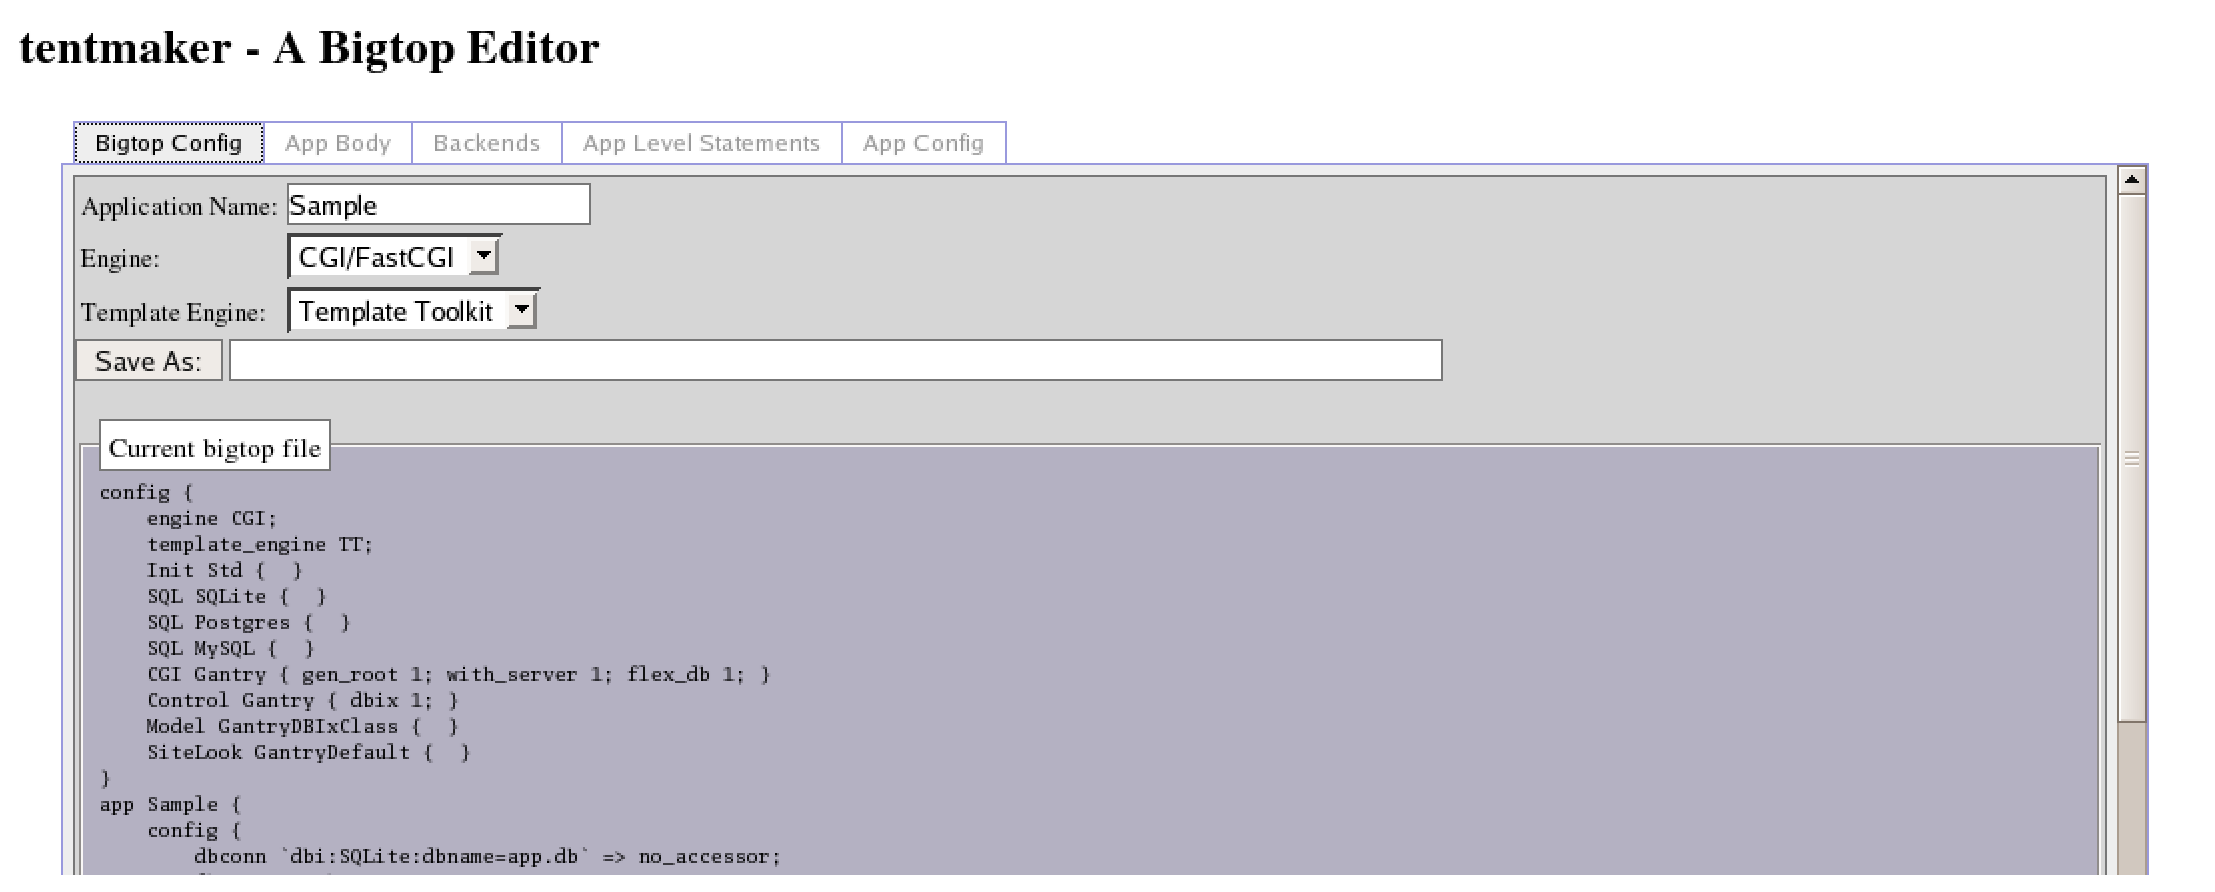
\includegraphics[width=6in]{tentopening}
\caption{The opening appearance of tentmaker.}
\label{fig:tentopening}
\end{figure}

There are five tabs which let you describe your app:

\begin{tabular}{l|l}
Tab Label & Allows you to specify... \\
\hline
Bigtop Config &
    the name of the app and a choice of engines which will serve it \\

App Body &
    the meat of your app, i.e. your tables and controllers \\

Backends &
    the list of all things bigtop should make for you, use check boxes \\
 &  to choose what you want it to do, and input boxes to configure \\
 &  each backend's output \\

App Level Statements &
    author names, their email addresses, project license, etc., all of \\
 &  these have nice defaults \\

App Config &
    a single input table for configuration of your app \\
\end{tabular}

We'll eventually visit all of the tabs in Chapter \ref{chap:tentref},
for now let's concentrate on making our address book work as my wife might
expect.  With that in mind the only thing of current interest on tentmaker's
opening page is the Save As button and the file name next to it.
Once we make our changes, we will return to this tab to press the button.

There are two issues we need to address: the columns in our table and
the database we are using.

To change the column names and add some new ones, click on the `App Body'
tab.  There you will see something similar to Figure \ref{fig:appbody}.

\begin{figure}
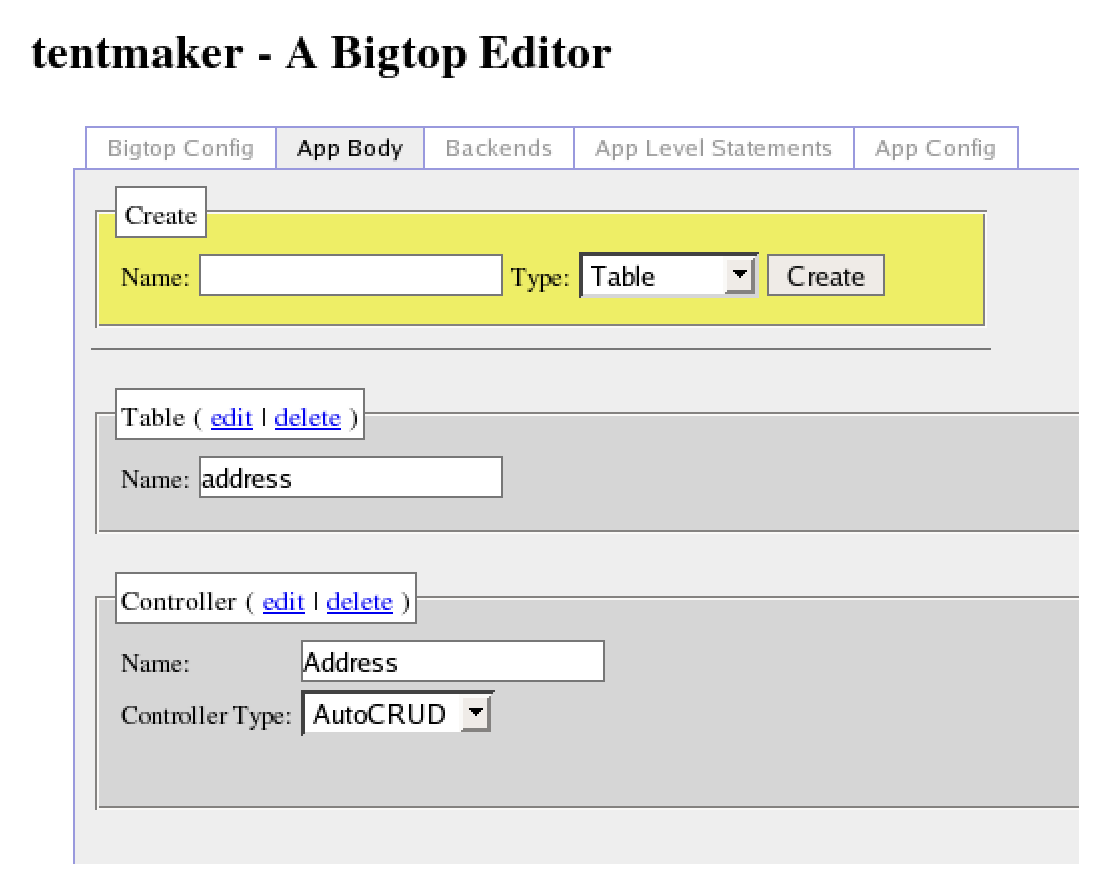
\includegraphics[width=6in]{appbody}
\caption{The App Body tentmaker tab for the address book example.}
\label{fig:appbody}
\end{figure}

We need to change the table and its controller to reflect our column
name preferences.  Start by clicking `edit' for the address table.
This will expand to show the statements and columns defined for the
table, as shown in Figure \ref{fig:tableedit}.

\begin{figure}
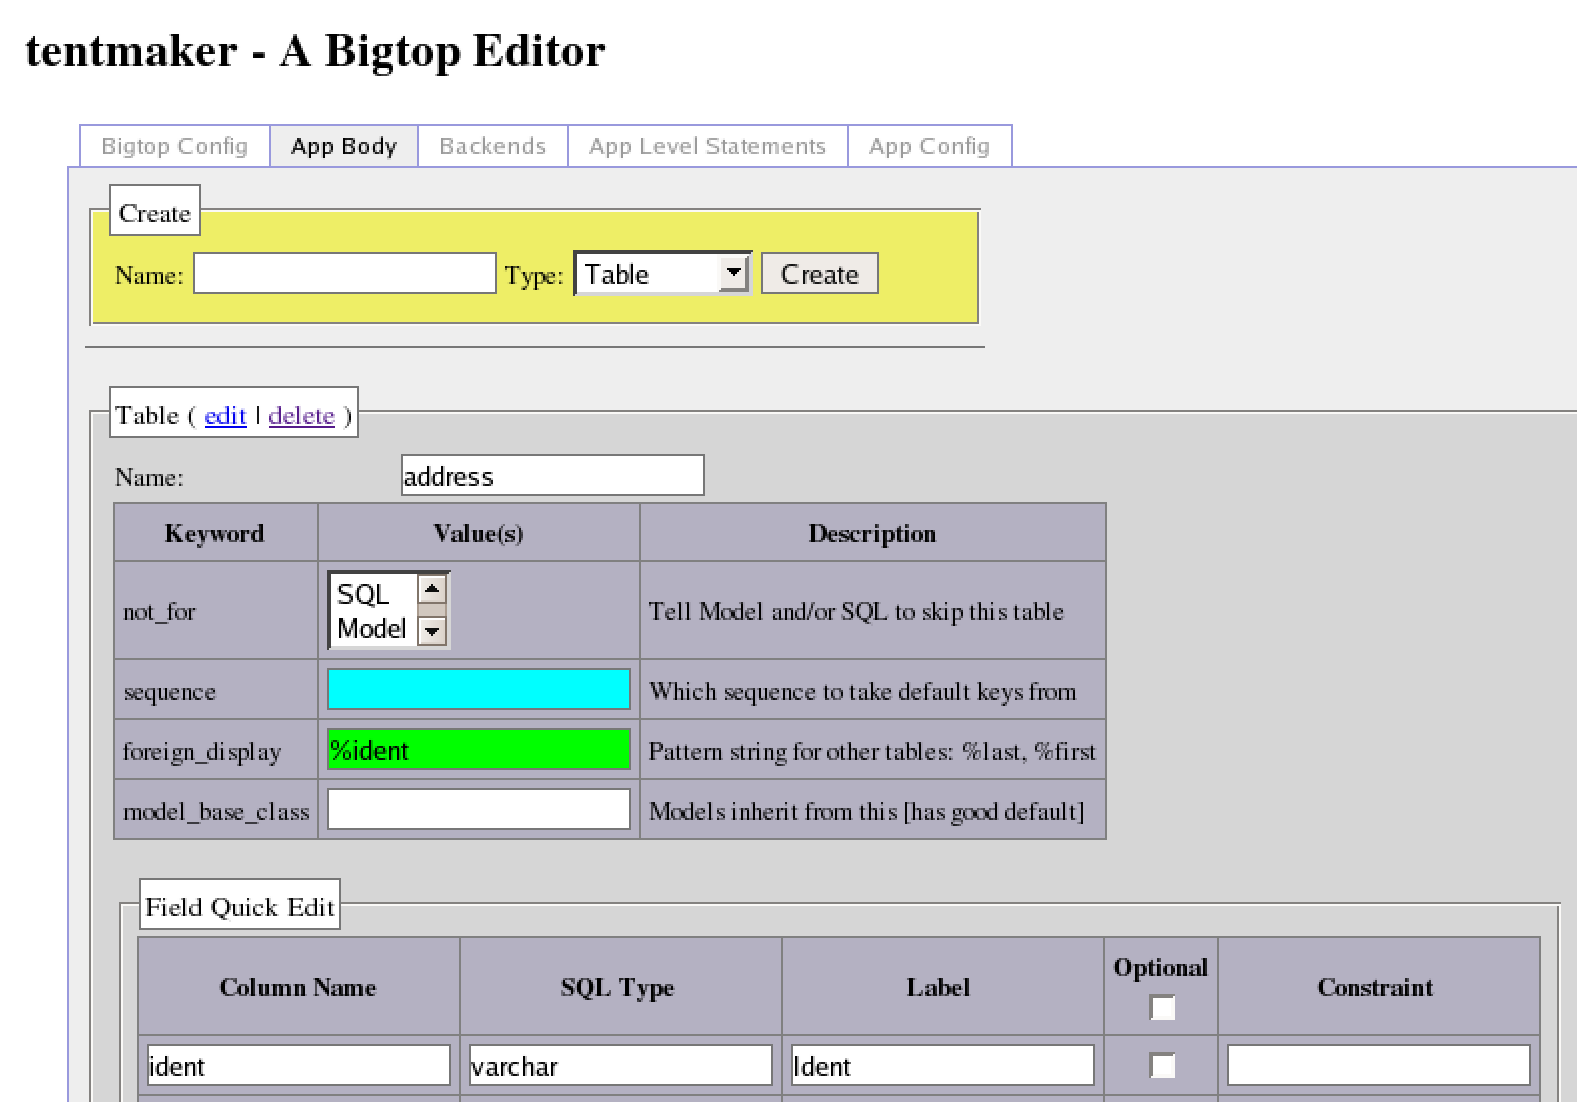
\includegraphics[width=4in]{tableedit}
\caption{Editing a table in tentmaker.}
\label{fig:tableedit}
\end{figure}

You may click edit again, at any time, to collapse the edit box.

First, scroll down in the tabbed pane to the Field Quick Edit
table shown more clearly in Figure \ref{fig:quickedit}.

Our original bigtop generation gave us five columns: id, ident, description,
created, and modified.  The last two are dates in case we want to start
tracking changes.  At least that would give my wife some clue of
address quality.  For now, we'll just ignore those.

The id is a unique primary key assigned by the database.  We can leave
it alone too.  That leaves the dreaded default columns ident and description.
Let's start by changing their names to `name' and `number.'  Just click
into the text fields under the `Column Name' label to do that.  To apply the
changes, click anywhere outside of the input box.  If you can't think
of a better place, feel free to click on the apparently useful
`Apply Quick Edit' button.

This is a good time to add additional fields for address information.
Add these by entering their names into the Create Field box and pressing
the button.  My table has these: address, city, state, zip, and email.
Add any that make sense to you.  Note that you can add as many fields as you
like at once by typing their names, separated by spaces, into the Name(s)
box.

When tentmaker makes a new field for you, it gives it a corresponding
label.  It does that by splitting the name at each underscore
and capitalizing the first letter of each resulting word.
The same things happens when you change the name of a field, if the
old label was formed that way.  If any of those labels looks odd -- perhaps
you prefer `email' to `Email' -- you can change them by typing your choice
into an input box under the `Label' heading.

If the new field should store something more interesting than text, you'll
also need to provide an SQL type for it in the SQL Type column.

Note that there is no reason to change the type from varchar, even if
your database needs something more specific.  The bigtop backend for your
database will magically convert it into something sensible.  If you object
to magic, supply the type of your choice.

Now save the bigtop file and regenerate:

\begin{verbatim}
bigtop docs/addressbook.bigtop all
\end{verbatim}

\subsection*{Dealing with Databases}

Before we restart our app.server, we need to address the database.
The one we used previously will not work, since the app now expects
different column names and more columns.

Since SQLite didn't support table alterations at the time of this writing
(at least not in a production version), we can't keep using the one we
-- or bigtop -- originally built.  This opens the subject of database
support and connection.

For now, we'll rely on the app.server to handle this for us.  See Chapter
\ref{chap:deploy} for how to handle it with CGI/FastCGI or \verb+mod_perl+.

Bigtop supports three databases:
SQLite, Postgres, and MySQL.  Its default generation assumes SQLite,
because it is so easy to work with during initial development.
But its defaults actually make the SQL needed to build the database in
Postgres and MySQL as well.  All of the SQL commands are in the
docs subdirectory of the build directory in files called schema.*,
where the asterisk is replaced with the database name.

If you want to stick with sqlite -- which is the easiest route -- delete
the old app.db, make a new one, and restart app.server:

\begin{verbatim}
sqlite app.db < docs/schema.sqlite
./app.server
\end{verbatim}

For Postgres this process goes like this (adjust the user names and
supply database passwords as needed):

\begin{verbatim}
createdb app.db -U postgres
psql app.db -U regular_user < docs/schema.postgres 
./app.server -d Pg -u regular_user -p password
\end{verbatim}

For MySQL it goes like this (again, adjust the user names and supply
database passwords as needed):

\begin{verbatim}
mysqladmin create app.db -u root -p
mysql -u regular_user -p app.db < docs/schema.mysql
./app.server -d mysql -u regular_user -p password
\end{verbatim}

Regardless of which database engine you use, you can change the name of
the database app.server will use with the -n flag (short for --dbname).

Of course, you could also edit app.server so it uses different defaults.
If you do that, remember to uncheck the `Build Server' box for the
CGI Gantry backend on the `Backends' tab in tentmaker.  Otherwise, whenever
you run bigtop, you changes will be overwritten.

\subsubsection*{Dealing with schema changes}

As development proceeds, data model changes are all but inevitable.
That is really the point of bigtop and its tentmaker editor.  Those
tools help with all the code and schema changes.  But there is one
thing they can't do: alter your database.

Every time I get tool envy about automated schema alterations, my
colleagues talk me out of working on the problem.  They always assert
that they wouldn't trust a tool to make production database alterations
under any circumstances.  Until they change there minds, their probably
won't be a schema change component to bigtop.

But, there is one thing bigtop can do to lessen the pain of data model
changes during development.  You can include literal SQL in the bigtop
file which will go directly into the generated docs/schema.* files
(at present all of them always receive the same SQL).  There is also
a table level data statement.  You can enter as many of these
as you like for any table.  Each one generates an INSERT INTO statement
for its table.  Combining literal SQL with data statements you can
have a nice, fresh database full of all sorts of lovely test data
simply by blowing away your old database and building a new one as shown
above.  Bigtop::Docs::Syntax explains both of these options (searching
there for `literal' or `data' is surprisingly effective).

There are also question/answer pairs about initial data in
Bigtop::Docs::Cookbook.  Look for, `How can I include initial data in a table?'
and `How do I put extra things into schema.*?'

\section{Interlude: Is this really required?}

To make further changes, we can revisit the bigtop file with tentmaker
or a text editor, save the result, and regenerate the app as shown above
(always being careful to alter or replace the database as needed).  For
example, Upon running the new version, I remembered that by default, all
fields are required.  But, Lisa's poor little fingers may not want to type
in all the data for each contact in her book -- she might not even know
most of it for most people.  So, we want to use tentmaker to make the fields
optional on the add and edit form.

Stop the app.server script (if it's still running).  From the build directory,
restart tentmaker, again giving it the existing bigtop file:

\begin{verbatim}
tentmaker docs/addressbook.bigtop
\end{verbatim}

(Remember to provide --port=... if needed.)

Click on the `App Body' tab so we can mark fields as optional in the address
table.  Click on the `address' table's `edit' link.  Lisa wants address,
city, state, zip, phone, and email to be optional (that's right, only name
will be required).  So, we should check the Optional box for
all the fields except name (and possibly phone) in the tentmaker.
We can also do this for all the fields by checking the Optional box in the
heading row.  Then, we can uncheck the ones we want to require, like the
name.

As a final touch, I think it would be a good idea to show the email address
next to the phone number on the main listing.  While still in tentmaker,
scroll down to the controller called Address.  You should see something
like Figure \ref{fig:controledit}.

\begin{figure}
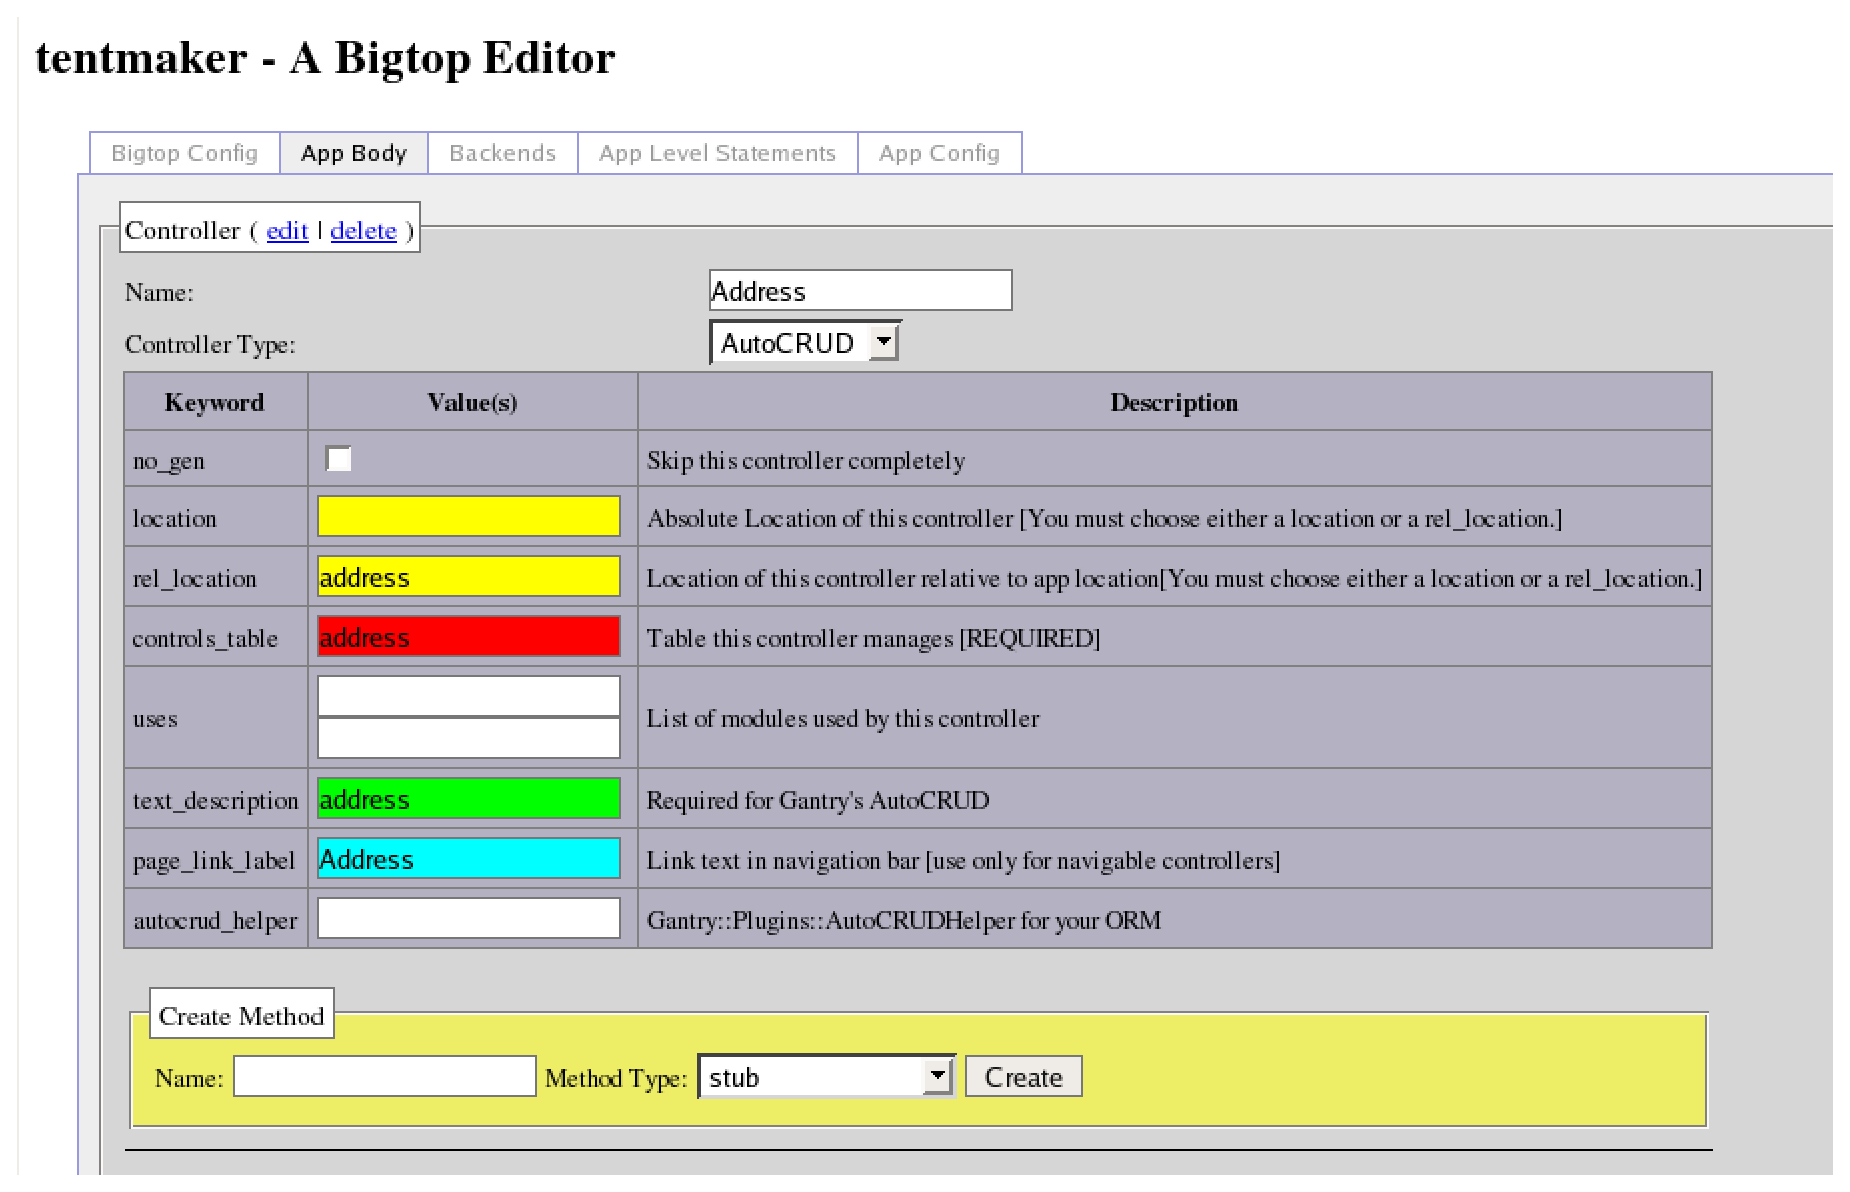
\includegraphics[width=4in]{controledit}
\caption{Editing a table in tentmaker.}
\label{fig:controledit}
\end{figure}

From there look for the method called \verb+do_main+ and edit it as
shown in Figure \ref{fig:mainlistedit}.  Add `email' below `number'
in a \verb+cols+ box.

Save the bigtop file.  Then stop the tentmaker and rebuild the app:

\begin{verbatim}
bigtop docs/addressbook.bigtop all
\end{verbatim}

Since we didn't make changes to the database, we can restart the app
immediately.

\begin{verbatim}
./app.server
\end{verbatim}

(Use whatever command line flags you used before.)

Note that the app.server always looks for your code in the lib subdirectory
of the build directory.  It never looks in blib/lib, so there is no
reason to run Build.PL at this point (unless you want to run the default
tests).

\section{Take Two: Should I send a card?}
\label{sec:asciiart}

Now, let's look at a more interesting exercise in that old address book.
On the back end paper, Lisa has scribbled some birth dates.
Perhaps including those dates in our present app will improve our on-time
arrival percentage for cards and gifts (and then again perhaps not).
It will certainly show off a few features of Gantry and Bigtop.

To add a table, we can ask tentmaker to augment the existing bigtop file
during start up:

\begin{verbatim}
tentmaker -a docs/addressbook.bigtop 'bday->address'
\end{verbatim}

This not only adds the table, but gives it a foreign key pointing to the
address table.  All we need to do from there is change each column name
of the new bday table to something more evocative and make sure they have
the proper `SQL Type.'

Here are all the ASCII art operators and what they mean:

\begin{tabular}{l|l|l}
Operator   & Example & Meaning \\
\hline
\verb+->+  & book->author   & book has a foreign key pointing to author \\
\verb+<-+  & author<-book   & book has a foreign key pointing to author \\
\verb+-+   & user-extrainfo & user and extrainfo have foreign keys to   \\
           &                & each other                                \\
\verb+<->+ & fox<->sock     & fox and sock share a many-to-many relationship\\
\end{tabular}

You can use exactly the same -a flag with bigtop -- and you can use -n
with tentmaker, just like we originally did with bigtop.  Always keep in
mind that using -n or -a with bigtop will automatically rebuild the
application, while tentmaker never rebuilds at all.  Every time you
save your changes in tentmaker, you need to run \verb+bigtop file.bigtop all+
for them to affect the application.

New tables are created in the order they are listed, so \verb+->+ and
\verb+<-+ are synonyms except for the table creation order.

Note that while existing tables mentioned in ASCII art are not recreated,
they will be receive new foreign keys or many-to-many relationships.

With the tentmaker restarted and the new table in place, let's start
by editing the column names for the new bday table, just as we did for
the address table.  Edit the table, change the names of the ident and
description fields.

All that remains is to make the date selectable.  Change the SQL Type of
the birth day field -- whatever you called it -- to date.

After you regenerate the app, there should be a new navigation tab
labeled \verb+Birth Days+ (or some other phrase according to your table name).
Go to it, to start entering birth days.

In this chapter we have seen how to use tentmaker to create a two table
web app for which we didn't have to write any code manually.  The next
chapter explains how to move this app into a \verb+mod_perl+ environment
with or without using Gantry::Conf to manage the configuration information.

Alternatively, now that we have seen how to use tentmaker modify generated
apps, you are ready for a more thorough tour.  If you want to take it now,
go to Chapter \ref{chap:tentref}.
